\documentclass[12pt,a4paper]{article}
\usepackage[utf8]{inputenc}
\usepackage[spanish,es-sloppy]{babel}
\usepackage{amsmath}
\usepackage{amsfonts}
\usepackage{amssymb}
\usepackage{graphicx}
\usepackage{tcolorbox}
\usepackage{here}
\usepackage{tikz}
\usepackage{pgfplots}
\usepackage[left=1.8cm,right=1.8cm,top=1.5cm,bottom=1.5cm]{geometry}
\usepackage{verbments}
\newcommand{\mrm}{\mathrm}
%\definecolor{fondo1}{rgb}{0.9764, 0.9764, 0.9762}
%\definecolor{fondo2}{rgb}{0.1647, 0.4980, 0.7}
\definecolor{fondo1}{rgb}{0.88, 0.88, 0.88}
\definecolor{fondo2}{rgb}{0.15, 0.15, 0.5}
\author{Josue Huaroto Villavicencio - 20174070I\\Sección: E}
\title{5$^{\circ}$ Práctica de Cálculo por Elementos Finitos - MC516}
\begin{document}
\fvset{frame=bottomline, framerule=0.02cm,numbers=left, numbersep=8pt}
\plset{language=python,texcl=true,listingnamefont=\sffamily\bfseries\color{white},captionbgcolor=fondo2, bgcolor=fondo1,listingname=\textbf{Código}, captionfont=\sffamily\color{white},fontsize=\normalsize}
\tcbset{colframe=black!50!gray,colback=gray!20,colupper=black,fonttitle=\bfseries,nobeforeafter,center title}
\maketitle
%\tableofcontents
\section{Diagrama de flujo}
\begin{figure}[H]
    \centering
    \includegraphics[scale = 1.75]{Flow.pdf}
    \caption{Diagrama de flujo}
\end{figure}
\section{Análisis analítico}
De las ecuaciones de equlibrio de la estática:
\begin{align*}
    R_{1} &= -R_{2}\\
    R_{1} &= 200\\
    R_{2} &= -200
\end{align*}
Se halla los correspondientes diagramas de momento flector y de fuerza cortante.
\begin{figure}[H]
    \centering
    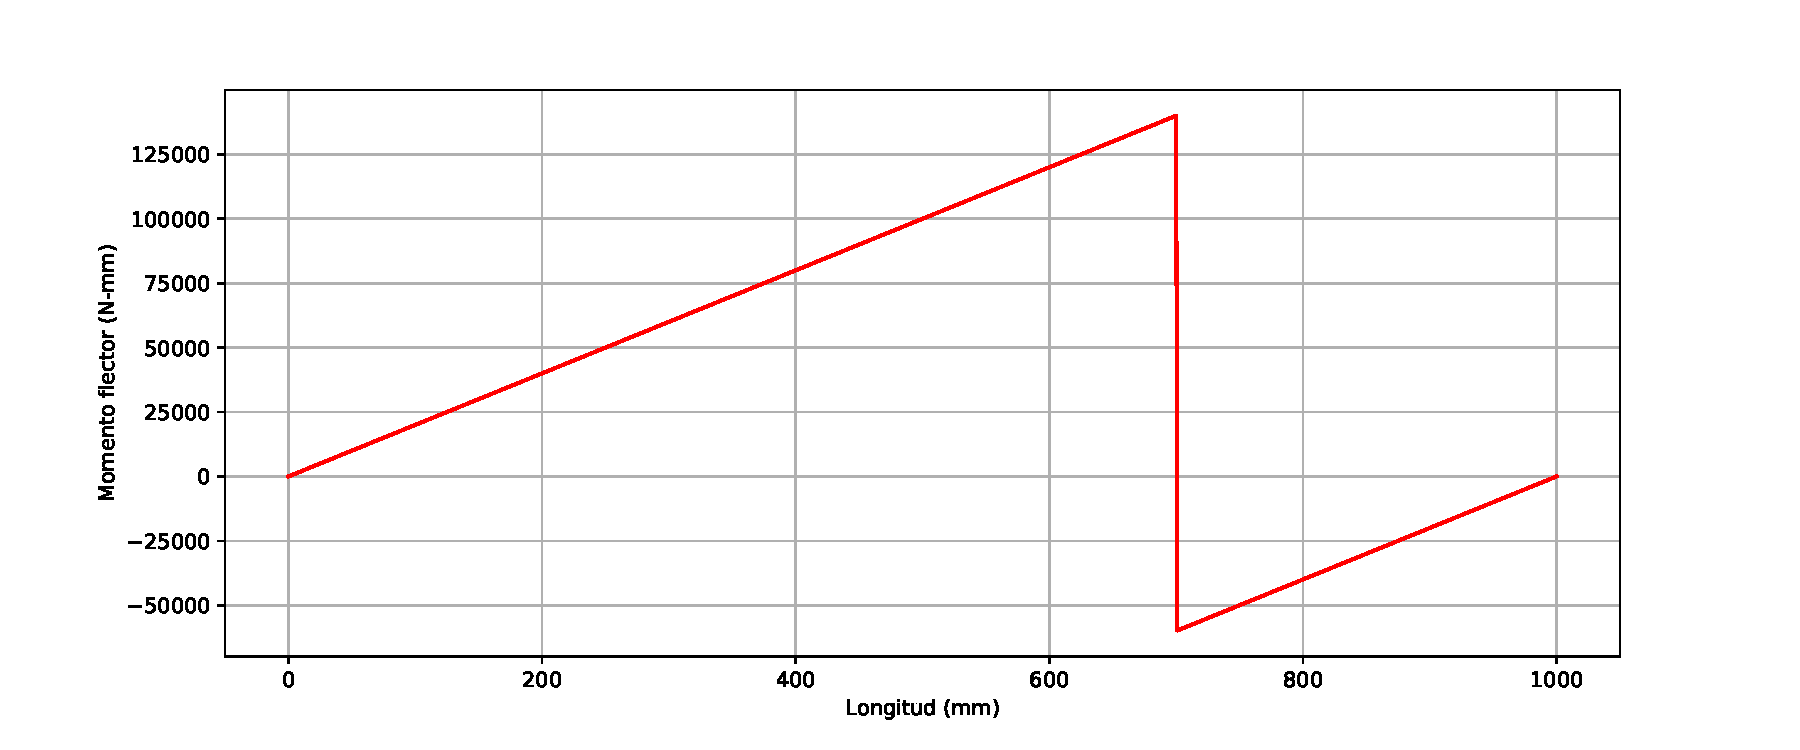
\includegraphics[scale=0.65]{dm.pdf}
    \caption{Diagrama de momento flector}
\end{figure}
\begin{figure}[H]
    \centering
    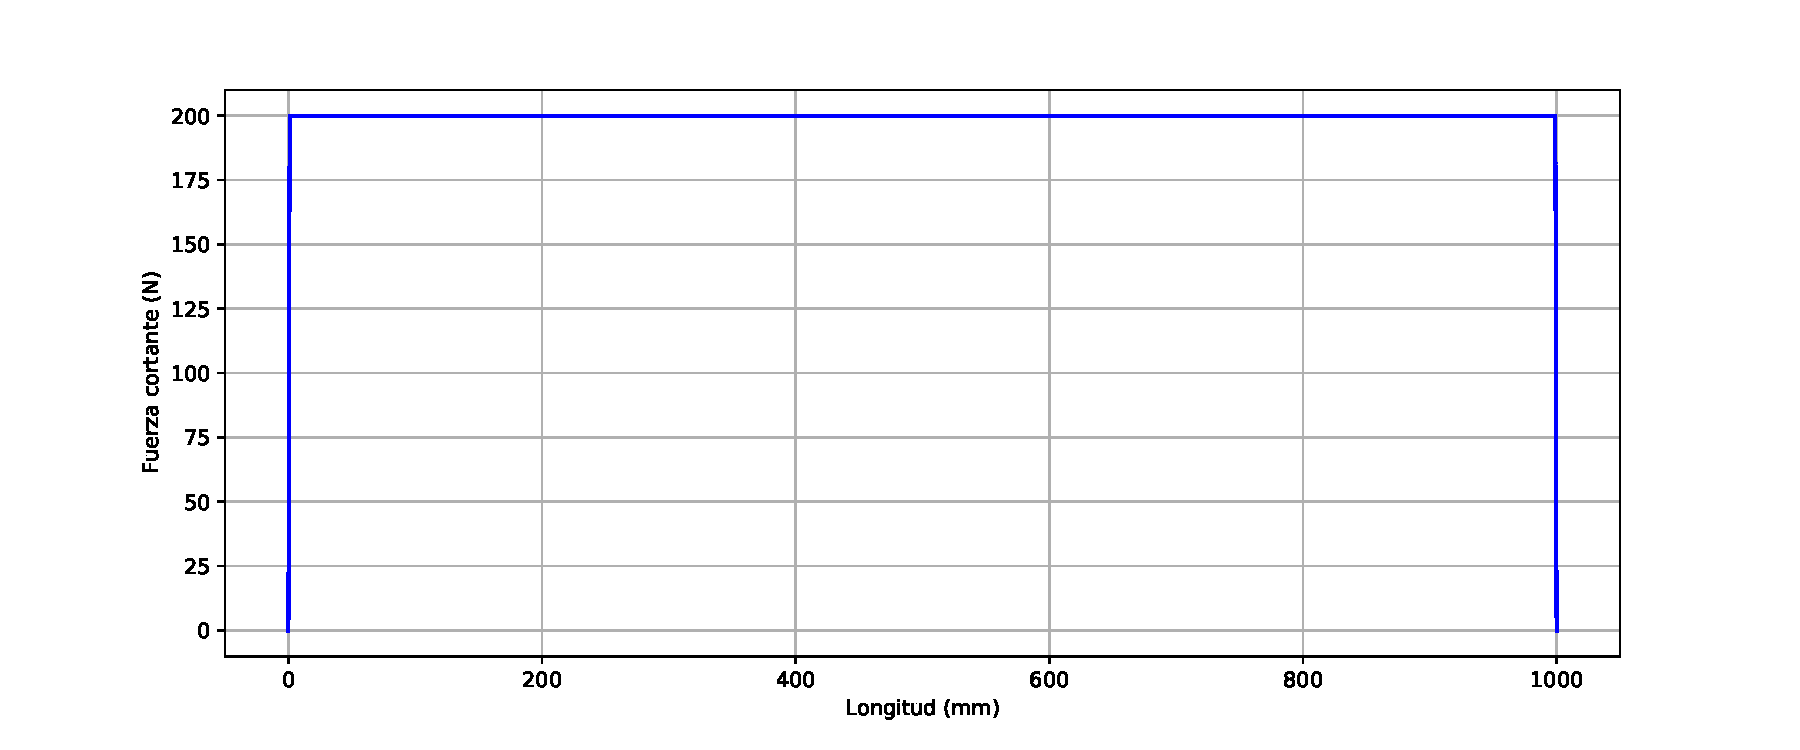
\includegraphics[scale=0.65]{dv.pdf}
    \caption{Diagrama de fuerza cortante}
\end{figure}
Luego, reescribiendo la función $M(x)$:
\begin{equation}
M(x) = R_{1}<x-0>^{1} - M <x-700>^{0} + R_{2} <x+1000>^{1}
\end{equation}
La ecuación diferencial correspondiente a la deformada de una viga:
\begin{align}
    EI\frac{\mrm{d}y^{2}}{\mrm{d}x^{2}} &= M(x)\\
    y(x) &= \frac{1}{EI}\iint M(x) \mrm{d}x \;\mrm{d}x\\
    y(x) &= \frac{\frac{R_{1}x^{3}}{6} + c_{1}x + c_{2}}{EI} \;\;\vert \;\; x \leq 700\\
    y(x) &= \frac{\frac{R_{1}x^{3}}{6} - \frac{Mx^{2}}{2} + c_{3}x + c_{4}}{EI} \;\;\vert \;\;x \geq 700
\end{align}
De las condiciones de frontera:
\begin{align}
    c_{2} &= 0\\
    c_{3} - 700M &= c_{1}\\
    c_{4} &= -49\times 10^{9}\\
    c_{3} &= 115666666.66667\\
    c_{1} &= -24333333.3333 \\
    y(x) &= \begin{cases}
    3.527337\cdot 10^{-11} x^{3} - 2.574956 \cdot 10^{-5}x & x \leq 700\\
    3.527337\cdot 10^{-11} x^{3} - 1.0582 \cdot 10^{-7} x^{2} + 1.224 \cdot 10^{-4}x - 0.051852 & x \geq 700
    \end{cases}
\end{align}
\begin{center}
\begin{tikzpicture}
\begin{axis}[
    height=7cm,
    width=16.5cm,
    axis lines = left,
    xlabel = Posición (mm),
    ylabel = {Deformada (mm)},
]
\addplot [
    domain=0:700, 
    samples=200, 
    color=red,
    line width=1.5,
]
{3.527337*10^(-11)*x^3-2.574956*10^(-5)*x};
\addlegendentry{$x \leq 700$}
\addplot [
    domain=700:1000, 
    samples=200, 
    color=blue,
    line width=1.5,
]
{3.527337*10^(-11)*x^3-1.0582*10^(-7)*x^2+1.224*10^(-4)*x-0.051852};
\addlegendentry{$x \geq 700$}
\end{axis}
\end{tikzpicture}
\end{center}
Derivando la ecuación (4), se obtiene el valor de la flecha máxima y su posición en la viga:
\begin{align*}
    x_{\max} &= 493.28828623 \\
    y_{\max} &= 0.00846797056
\end{align*}
Derivando la ecuación (11), se obtiene la gráfica de la pendiente de la deformada:
\begin{equation}
    \theta (x) = \begin{cases}
    10.582011\cdot 10^{-11} x^{2} - 2.574956 \cdot 10^{-5} & x \leq 700\\
    10.582011\cdot 10^{-11} x^{2} - 2.1164\cdot 10^{-7} x + 1.224 \cdot 10^{-4} & x \geq 700
    \end{cases}
\end{equation}
\begin{center}
\begin{tikzpicture}
\begin{axis}[
    height=7cm,
    width=16.5cm,
    axis lines = left,
    xlabel = Posición (mm),
    ylabel = {Pendiente},
]
\addplot [
    domain=0:700, 
    samples=200, 
    color=red,
    line width=1.5,
]
{10.582011*10^(-11)*x^2 - 2.574956*10^(-5)};
\addlegendentry{$x \leq 700$}
\addplot [
    domain=700:1000, 
    samples=200, 
    color=blue,
    line width=1.5,
]
{10.582011*10^(-11)*x^(2) - 2.1164*10^(-7)*x + 1.224*10^(-4)};
\addlegendentry{$x \geq 700$}
\end{axis}
\end{tikzpicture}
\end{center}
\section{Ejecución del código}
Se agrega al solver principal una nueva función llamada DFBoundaryCondition que se utilizará para agregar una fuerza distribuida sobre un elemento.
\begin{pyglist}[language=python,caption={Carga distribuida sobre un elemento},style=pastie]
def DFBoundaryCondition(nF,w,e):
    f = Elements[e][0]
    s = Elements[e][1]
    l = L[e]
    FBoundaryCondition(nF,w*l/2,2*f+0)
    FBoundaryCondition(nF,w*l*l/12,2*f+1)
    FBoundaryCondition(nF,w*l/2,2*s+0)
    FBoundaryCondition(nF,-w*l*l/12,2*s+1)
\end{pyglist}
Ahora, es necesario modificar la inserción de las matrices de rigidez de los elementos a la matriz de rigidez global.
\begin{pyglist}[language=python,caption={Ensamble de la matriz de rigidez},style=pastie]
def ElementStiffness(E, I, L):
    aux = np.zeros((4,4))
    s1 = np.array([12,6*L,-12,6*L])
    s2 = np.array([6*L,4*L*L,-6*L,2*L*L])
    for i in range(0,2):
        for j in range(0,4):
            aux[2*i][j] = s1[j]
            aux[2*i+1][j] = s2[j]
            if(i == 1):
                aux[2*i][j] *= -1
    aux[3][1] = 2*L*L
    aux[3][3] = 4*L*L
    aux = aux*E*I/(L**3)
    return aux

def AssemblyStiffness(nStiffnessMatrix,k,i,j):
    for p in range(0,2):
        for m in range(0,2):
            nStiffnessMatrix[2*i+p][2*i+m] += k[p][m]
            nStiffnessMatrix[2*i+p][2*j+m] += k[p][2+m]
            nStiffnessMatrix[2*j+p][2*i+m] += k[p+2][m]
            nStiffnessMatrix[2*j+p][2*j+m] += k[p+2][2+m]
\end{pyglist}
Todos los demás elementos del código permanecen igual; ahora solo se necesita definir las condiciones del problema a resolver.
\begin{pyglist}[language=python,caption={Condiciones del problema},style=pastie]
NodesCondition = []
Nodes = 1001
Nodes *= 2
NumberOfElement = 1000

E = 3e5 #MPA
K = []
I = 315e4 #mm$^{4}$
M_A = 2e5 #N-mm
PosNodes = np.arange(0,1000+1,1)
Elements = []
for i in range(0,1000):
    Elements.append((i,i+1))
Elements = np.array(Elements)

L = []
for i in range(NumberOfElement):
    L.append(PosNodes[Elements[i][1]] - PosNodes[Elements[i][0]])
L = np.array(L)

for i in range(0,NumberOfElement):
    aux = ElementStiffness(E,I,L[i])
    K.append(aux)


StiffnessMatrix = np.zeros((Nodes,Nodes))

U = np.zeros(Nodes).reshape(Nodes,1)
F = np.zeros(Nodes).reshape(Nodes,1)

Initialize(StiffnessMatrix,U,F)

#Node in UBoundary = Node*2+(y=0,phi=1)
UBoundaryCondition(U,0,2*0+0) #Nodo 0 en Y
UBoundaryCondition(U,0,2*1000+0) #Nodo 1000 en Y

#DFBC(F,w,element)
#FBC(F,f,Node*2+(y=0,phi=1))
FBoundaryCondition(F,M_A,2*700+1) #Momento en el nodo 700


U,F=Solve(StiffnessMatrix,U,F)
print("Stiffness Matrix:\n",StiffnessMatrix,'\n')
print("Displacements:\n",U,'\n')
print("Forces:\n",F)
\end{pyglist}

\section{Resultados del problema}
Al finalizar la ejecución del solver, obtenemos la matriz de rigidez, las fuerzas y desplazamientos:
\begin{figure}[H]
    \centering
    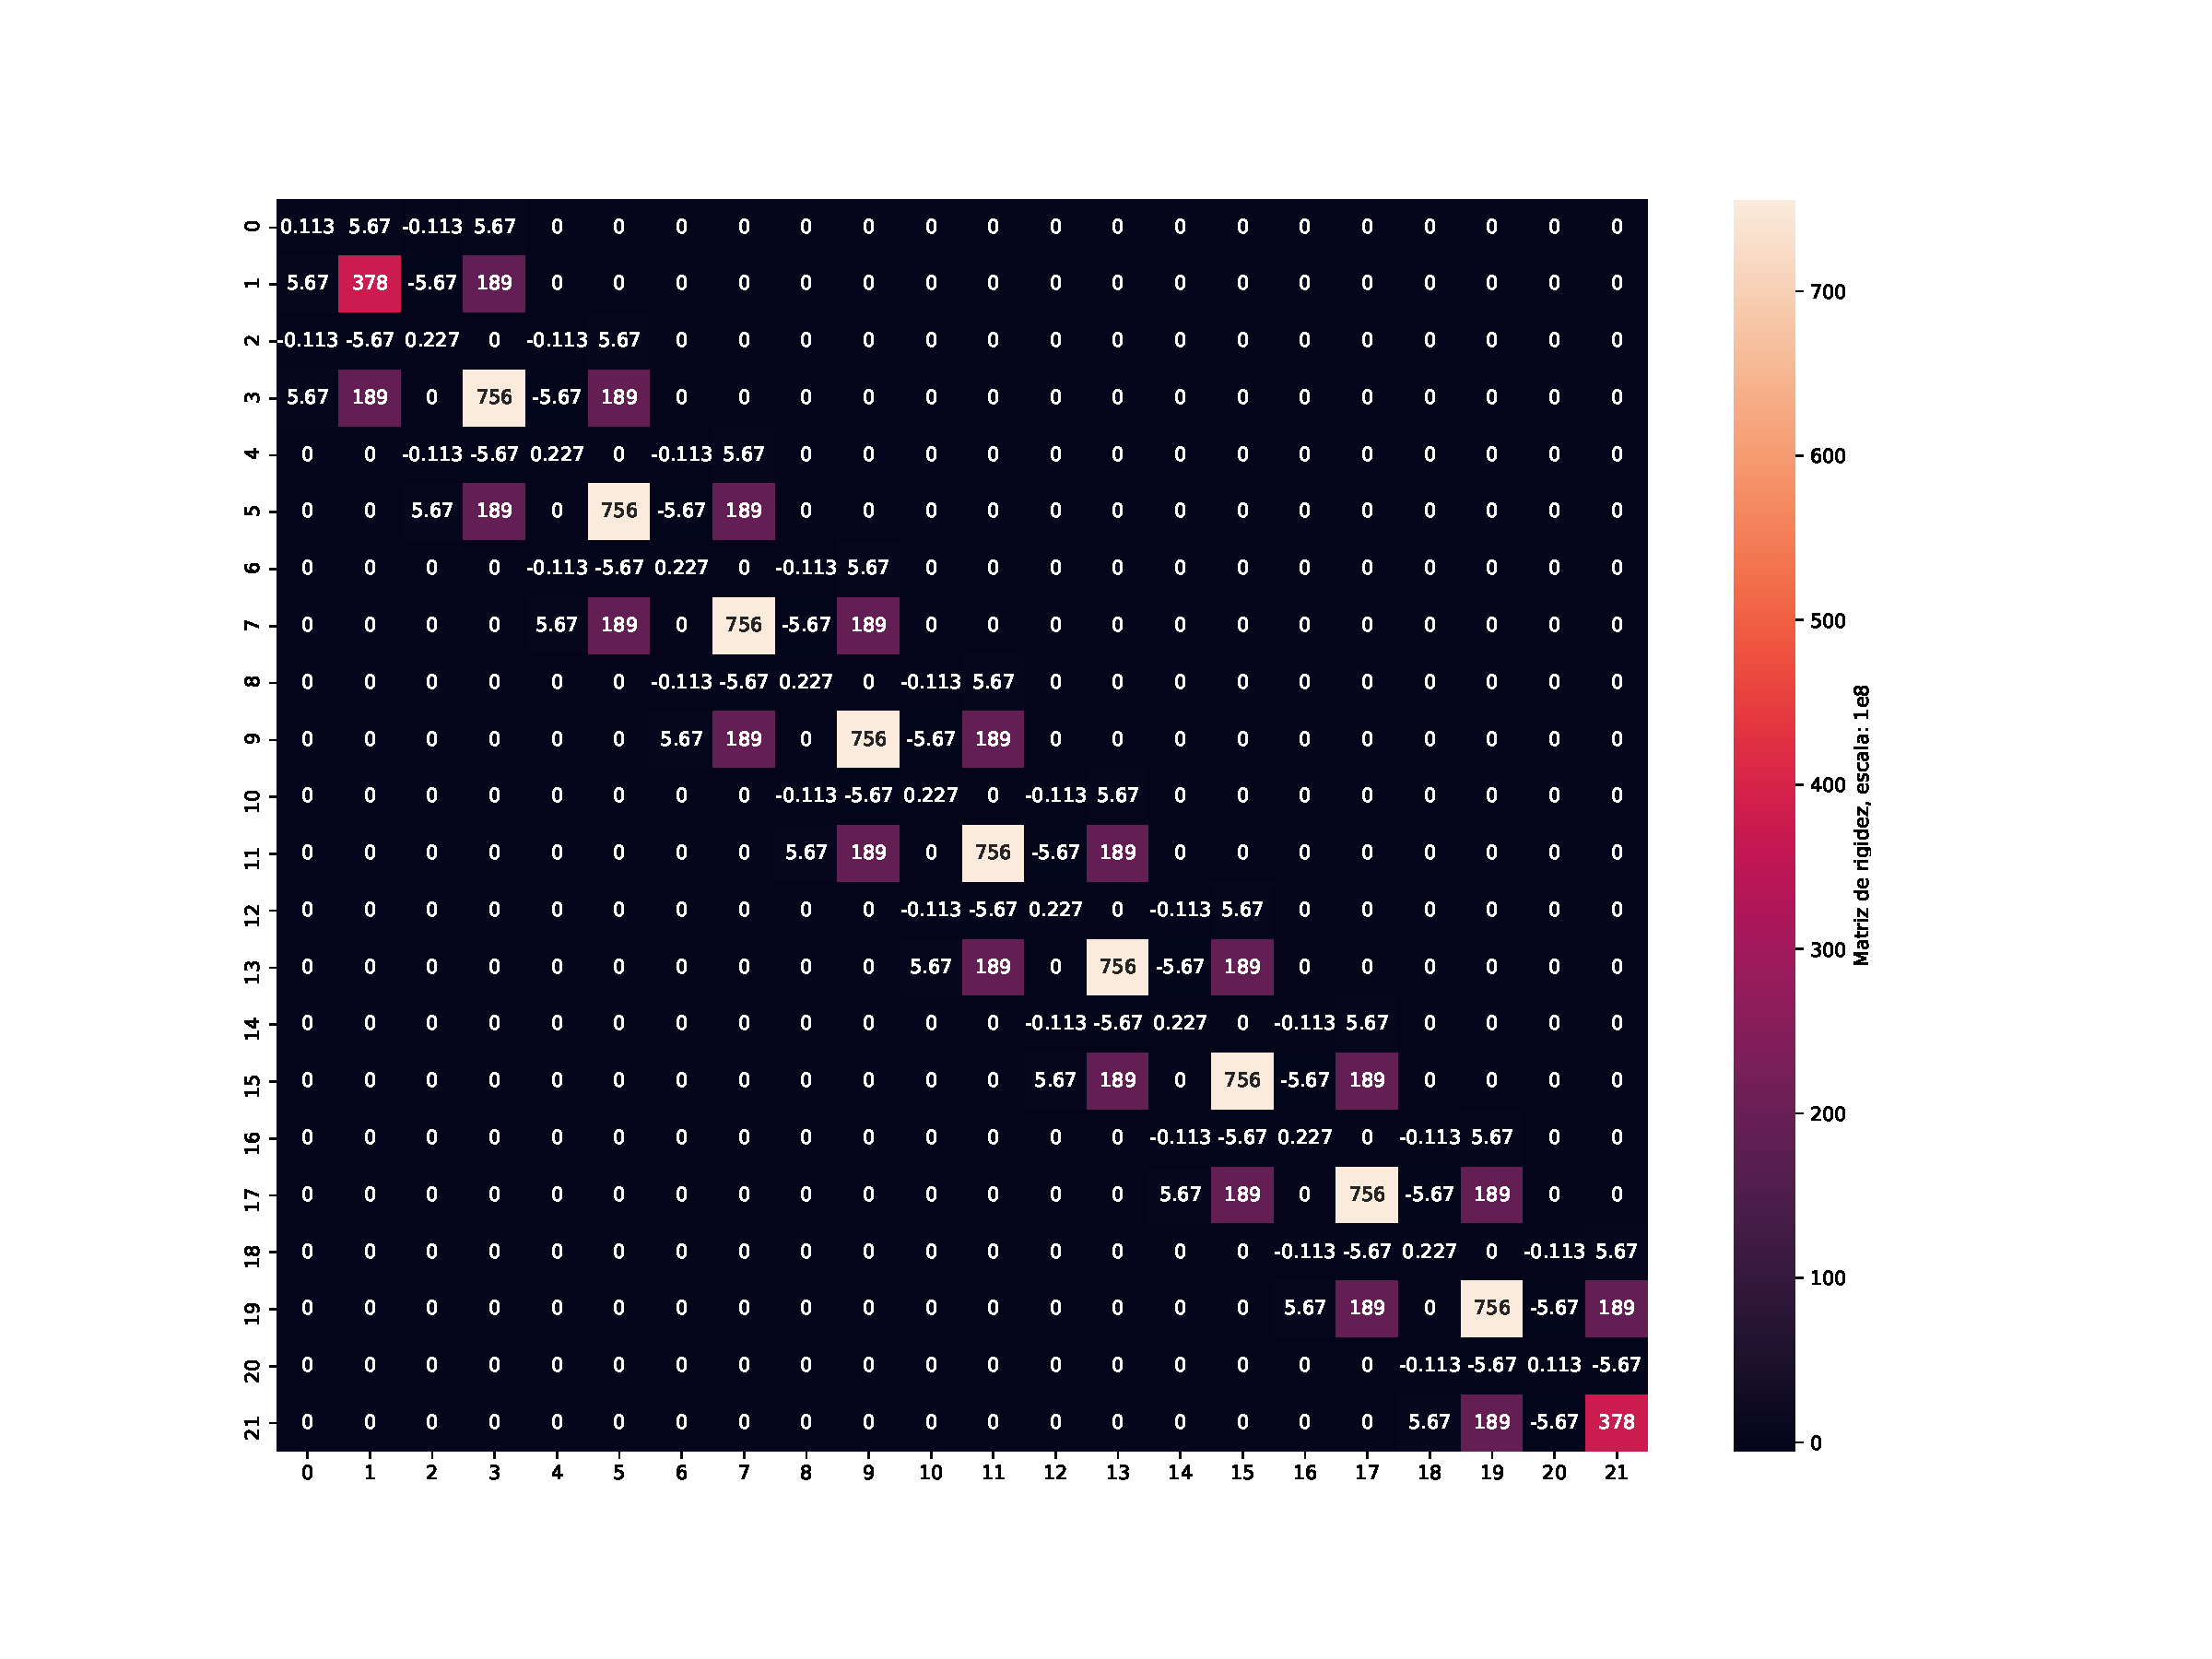
\includegraphics[scale=0.585]{stiffness.pdf}
    \caption{Matriz de rigidez}
\end{figure}
\begin{figure}[H]
    \centering
    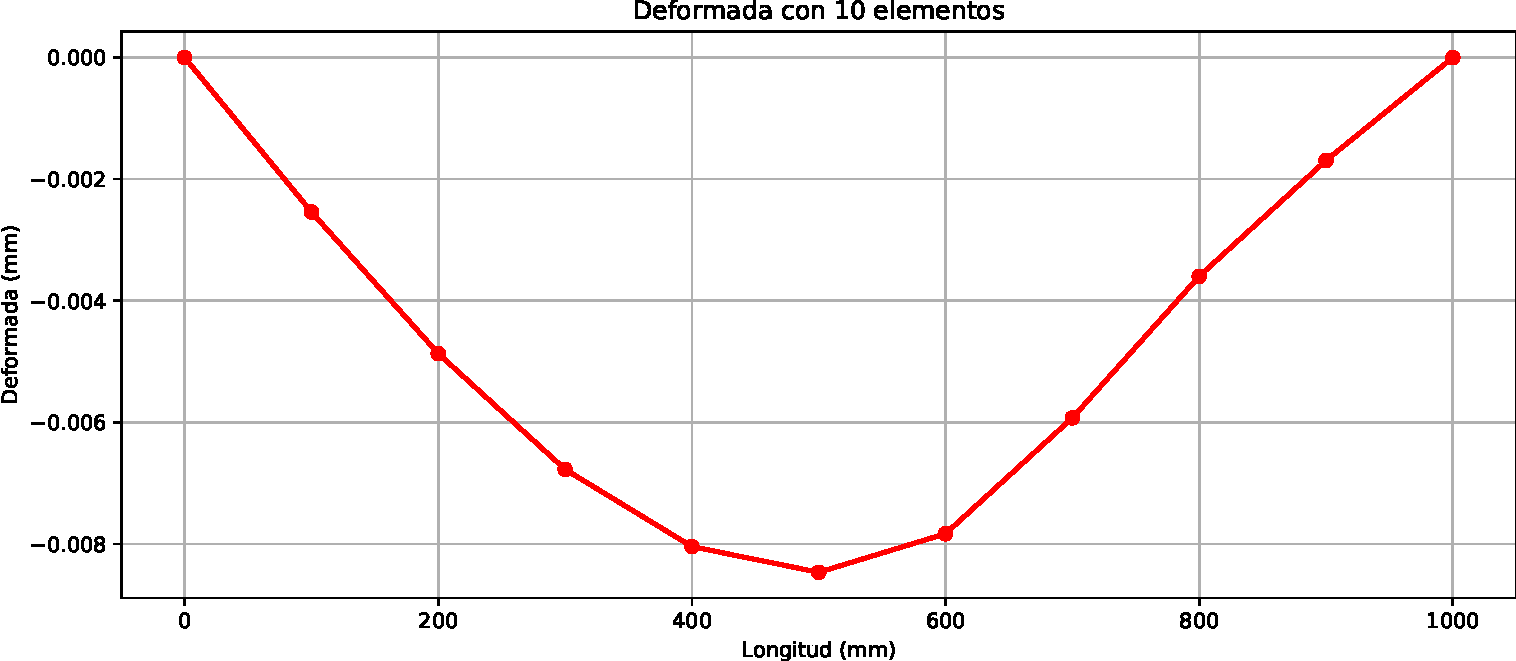
\includegraphics[scale=0.66]{displacements10.pdf}
    \caption{Deformada}
\end{figure}
\begin{figure}[H]
    \centering
    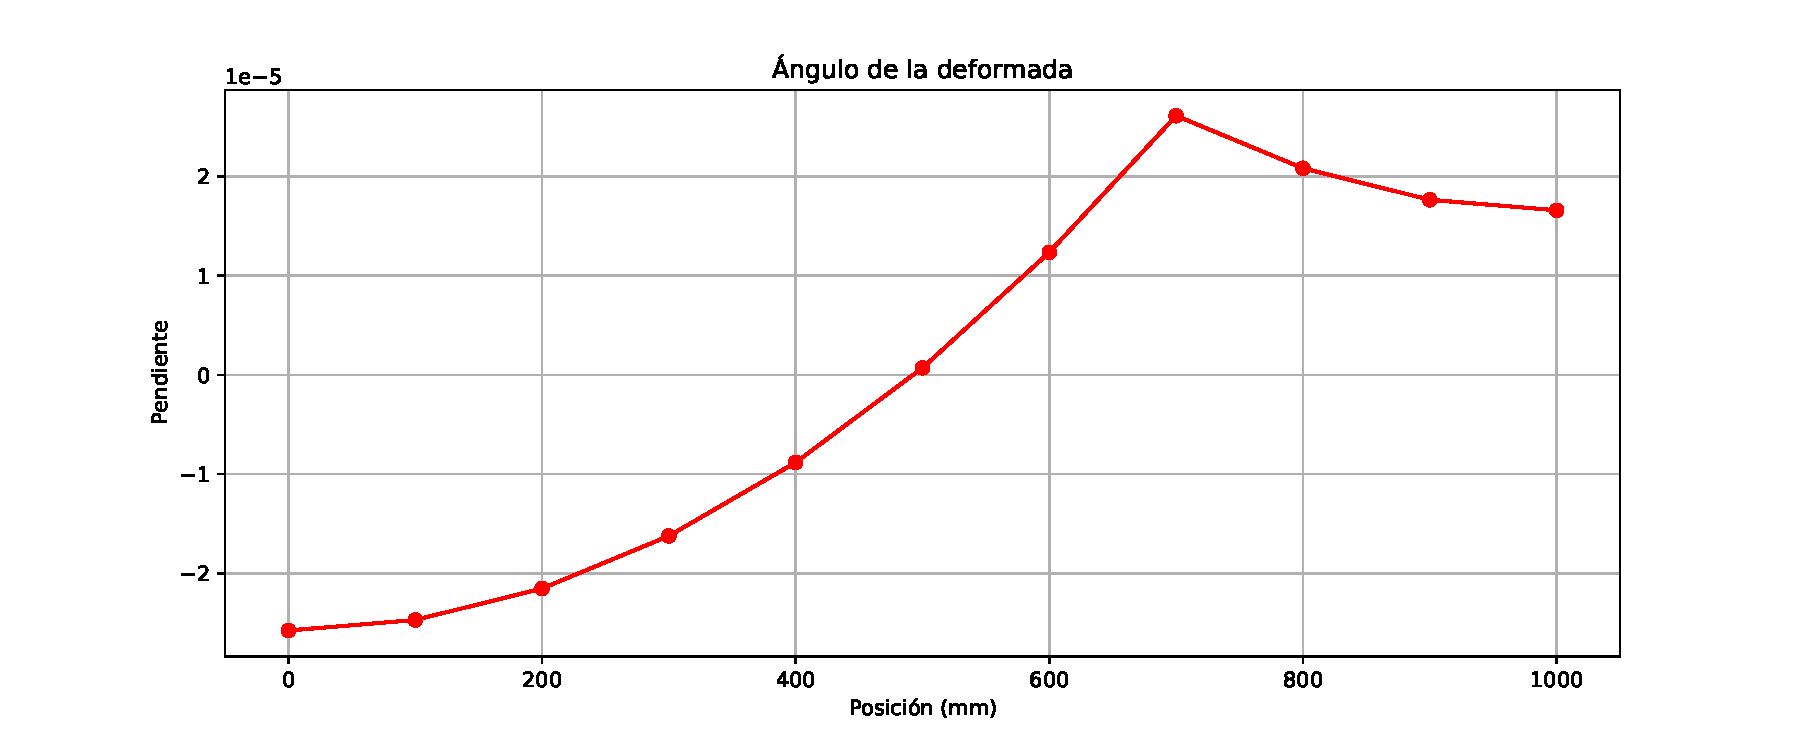
\includegraphics[scale=0.66]{angle10.pdf}
    \caption{Pendiente}
\end{figure}
Cada desplazamiento y fuerza corresponde a un nodo en una dirección ($y$ o $\theta$); por lo que al nodo $i$ le corresponde las reacciones $2i$ ($y$) y $2i+1$ ($\theta$).\\
Se organiza los datos del desplazamiento y fuerza en cada dirección en una tabla para cada nodo para tener una mejor compresión de los resultados:
\begin{table}[H]
    \centering
    \tcbox[left=0mm,right=0mm,top=0mm,bottom=0mm,boxsep=0mm,toptitle=0.8mm,bottomtitle=0.8mm,title=Resultados del análisis por elementos finitos]{
    \renewcommand{\arraystretch}{1.2}%
    \begin{tabular}{|c|c|c|c||c|c|c||c|}
        \hline
        Nodo & Desp. x (mm) & Desp. y (mm) & Desp. z (mm) & Fuerza x (N) & Fuerza y (N) & Fuerza z (N) & Fuerza resultante (N)\\
        \hline
        0 & 0.0 & 0.0 & 0.0 & -3403.09997 & 4374.50697 & 580.26842 & 5572.62165 \\
        \hline
        1 & -0.00607 & -0.04191 & 0.01043 & 0.0 & 0.0 & 0.0 & 0.0 \\
        \hline
        2 & -0.01075 & -0.03483 & 0.00254 & 0.0 & 0.0 & 0.0 & 0.0 \\
        \hline
        3 & -0.01474 & 0.0 & 0.0 & 0.0 & 1993.5736 & 98.79737 & 1996.0202 \\
        \hline
        4 & -0.00897 & -0.04223 & 0.01815 & 0.0 & -5000.0 & 0.0 & 5000.0 \\
        \hline
        5 & -0.00057 & -0.03471 & 0.00731 & 3758.77048 & -1368.08057 & 0.0 & 4000.0 \\
        \hline
        6 & 0.0 & 0.0 & 0.0 & -4114.441 & 4650.96484 & -679.06578 & 6246.69745 \\
        \hline
        7 & -0.00692 & -0.05129 & 0.01043 & 0.0 & 0.0 & 0.0 & 0.0 \\
        \hline
        8 & -0.01384 & -0.04263 & 0.00167 & 0.0 & 0.0 & 0.0 & 0.0 \\
        \hline
        9 & -0.01817 & 0.0 & 0.0 & 0.0 & 1717.11573 & 0.0 & 1717.11573 \\
        \hline
        10 & -0.01157 & -0.05129 & 0.01815 & 0.0 & -5000.0 & 0.0 & 5000.0 \\
        \hline
        11 & -0.00056 & -0.04204 & 0.00793 & 3758.77048 & -1368.08057 & 0.0 & 4000.0
    \end{tabular}}
    \caption{Desplazamientos y reacciones en los nodos}
\end{table}
Luego, los esfuerzos en cada elemento:
\begin{table}[H]
    \centering
    \tcbox[left=0mm,right=0mm,top=0mm,bottom=0mm,boxsep=0mm,toptitle=0.8mm,bottomtitle=0.8mm,title=Esfuerzos para los elementos de la armadura]{
    \renewcommand{\arraystretch}{1.2}%
    \begin{tabular}{c||c|c||c||c}
        Elemento & Nodo 1 & Nodo 2 & Longitud (mm) & Esfuerzo (MPa)\\
        \hline
        0 & 0 & 1 & 600.0 & -2.12568 \\
        \hline
        1 & 0 & 4 & 692.82032 & 4.04634 \\
        \hline
        2 & 0 & 6 & 500.0 & 0.0 \\
        \hline
        3 & 0 & 10 & 854.40037 & 0.505 \\
        \hline
        4 & 1 & 2 & 600.0 & -1.63612 \\
        \hline
        5 & 1 & 4 & 346.41016 & 0.19657 \\
        \hline
        6 & 1 & 6 & 781.02497 & 0.54023 \\
        \hline
        7 & 1 & 7 & 500.0 & 0.0 \\
        \hline
        8 & 1 & 8 & 781.02497 & -0.09704 \\
        \hline
        9 & 1 & 10 & 608.27625 & -0.34516 \\
        \hline
        10 & 2 & 3 & 600.0 & -1.39597 \\
        \hline
        11 & 2 & 4 & 692.82032 & 0.65348 \\
        \hline
        12 & 2 & 5 & 346.41016 & -0.07434 \\
        \hline
        13 & 2 & 8 & 500.0 & 0.3643 \\
        \hline
        14 & 2 & 10 & 854.40037 & -0.46391 \\
        \hline
        15 & 2 & 11 & 608.27625 & -0.11292 \\
        \hline
        16 & 3 & 5 & 692.82032 & 1.5422 \\
        \hline
        17 & 3 & 8 & 781.02497 & -0.47202 \\
        \hline
        18 & 3 & 9 & 500.0 & 0.0 \\
        \hline
        19 & 3 & 11 & 854.40037 & 0.60235 \\
        \hline
        20 & 4 & 5 & 600.0 & 2.9383 \\
        \hline
        21 & 4 & 10 & 500.0 & 0.0 \\
        \hline
        22 & 5 & 10 & 781.02497 & 0.40563 \\
        \hline
        23 & 5 & 11 & 500.0 & -0.25968 \\
        \hline
        24 & 6 & 7 & 600.0 & -2.42228 \\
        \hline
        25 & 6 & 10 & 692.82032 & 4.73743 \\
        \hline
        26 & 7 & 8 & 600.0 & -2.42228 \\
        \hline
        27 & 7 & 10 & 346.41016 & 0.0 \\
        \hline
        28 & 8 & 9 & 600.0 & -1.51471 \\
        \hline
        29 & 8 & 10 & 692.82032 & 0.71534 \\
        \hline
        30 & 8 & 11 & 346.41016 & -0.35767 \\
        \hline
        31 & 9 & 11 & 692.82032 & 1.74904 \\
        \hline
        32 & 10 & 11 & 600.0 & 3.85203
    \end{tabular}}
    \caption{Esfuerzos para los elementos de la armadura}
\end{table}
\section{Generalización para $\mathbf{n}$ elementos}
Al incrementar la cantidad de elementos se obtiene mayor información sobre la pendiente y la deformada en más secciones de la viga.
\begin{figure}[H]
    \centering
    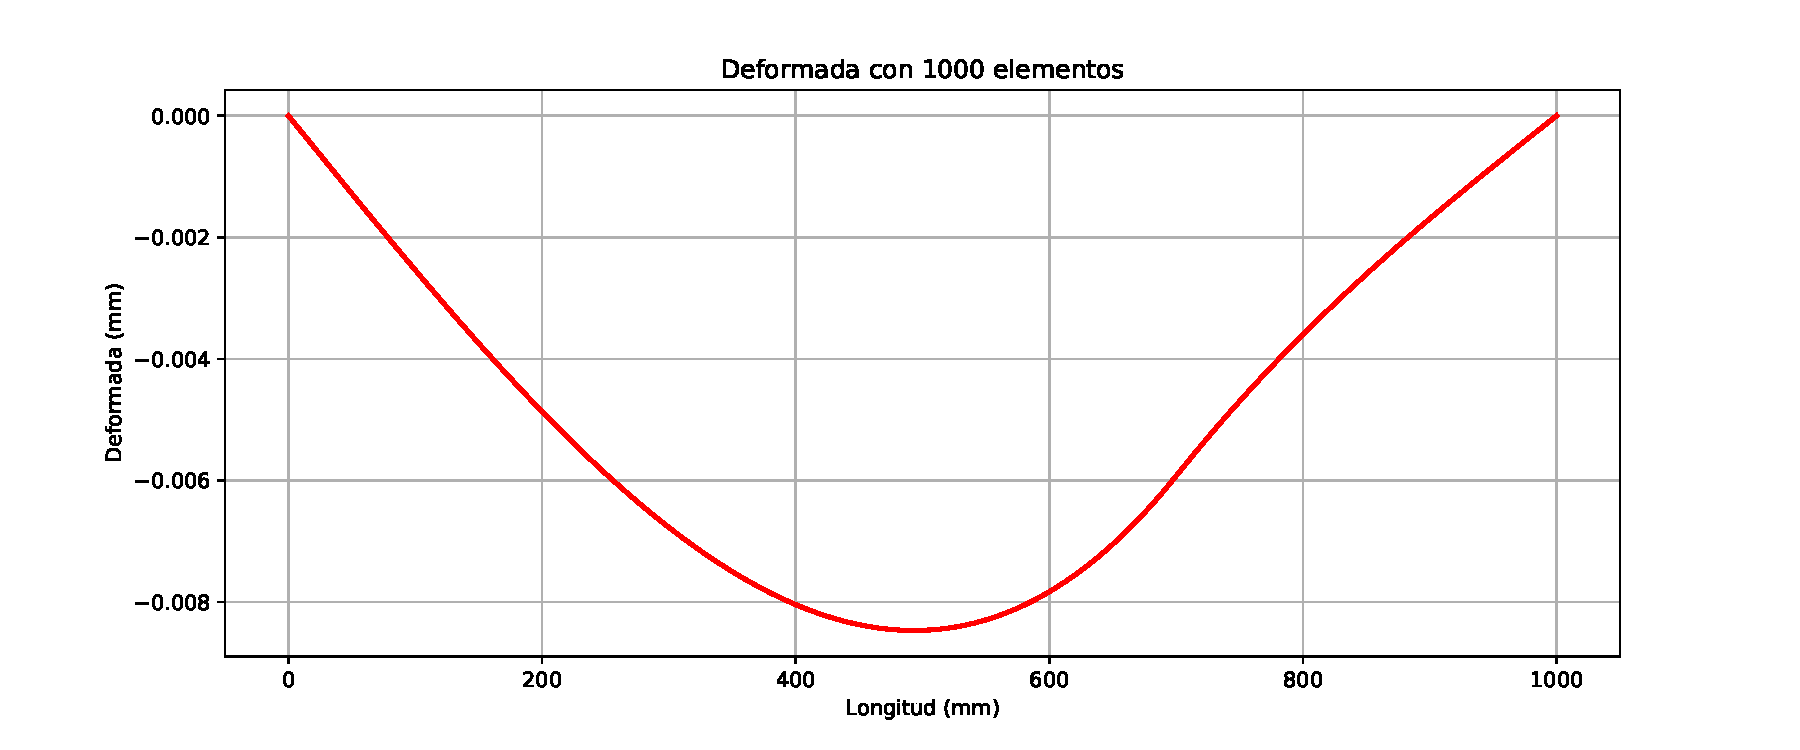
\includegraphics[scale=0.67]{displacements1000.pdf}
    \caption{Deformada para 1000 elementos}
\end{figure}
\begin{figure}[H]
    \centering
    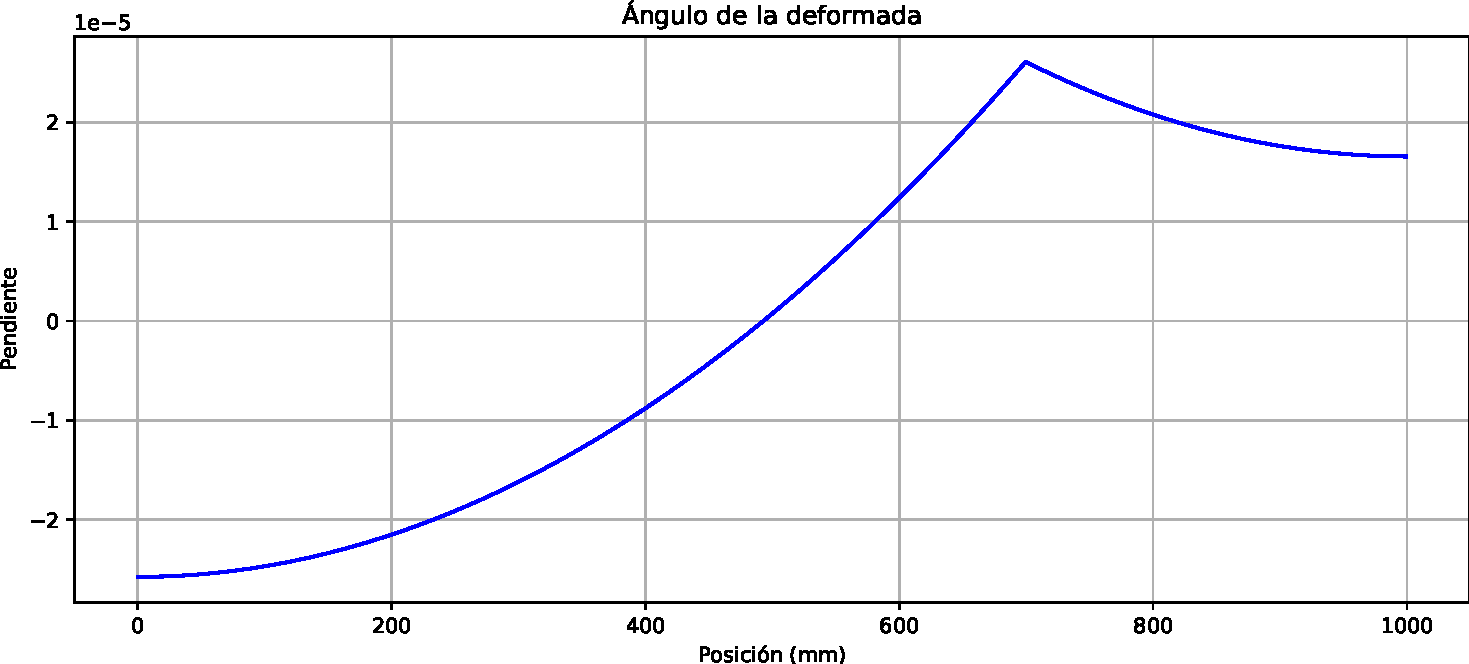
\includegraphics[scale=0.69]{angle1000.pdf}
    \caption{Pendiente para 1000 elementos}
\end{figure}

\section{Verificación de resultados}

\section{Conclusiones}

\section*{Anexos}
\subsection*{Convergencia del método de elementos finitos}
\begin{figure}[H]
    \centering
    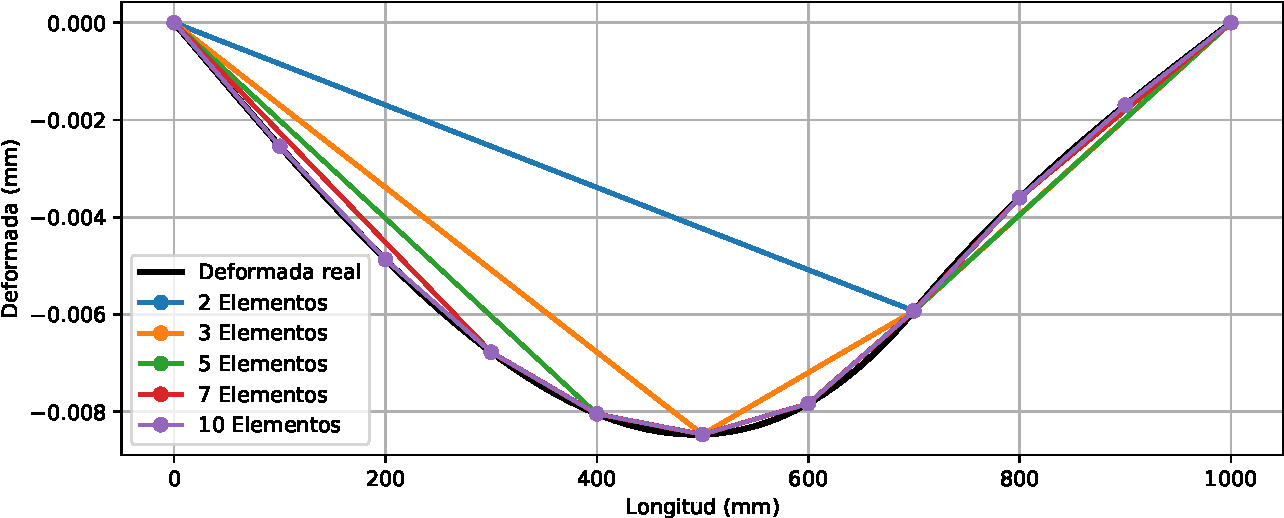
\includegraphics[scale=0.78]{comparision2.pdf}
    \caption{Convergencia de la deformada al aumentar los elementos}
\end{figure}
\subsection*{Optimización del mallado}
Se observa que la flecha máxima se encuentra entre 400 y 500 mm. Para obtener una mayor precisión de la ubicación de la flecha puede aumentarse el mallado, pero esto crearía demasiados elementos, entonces solo se mejora el mallado entre una región más pequeña, mientras que en las otras secciones de la viga el mallado sigue como antes.
\begin{figure}[H]
    \centering
    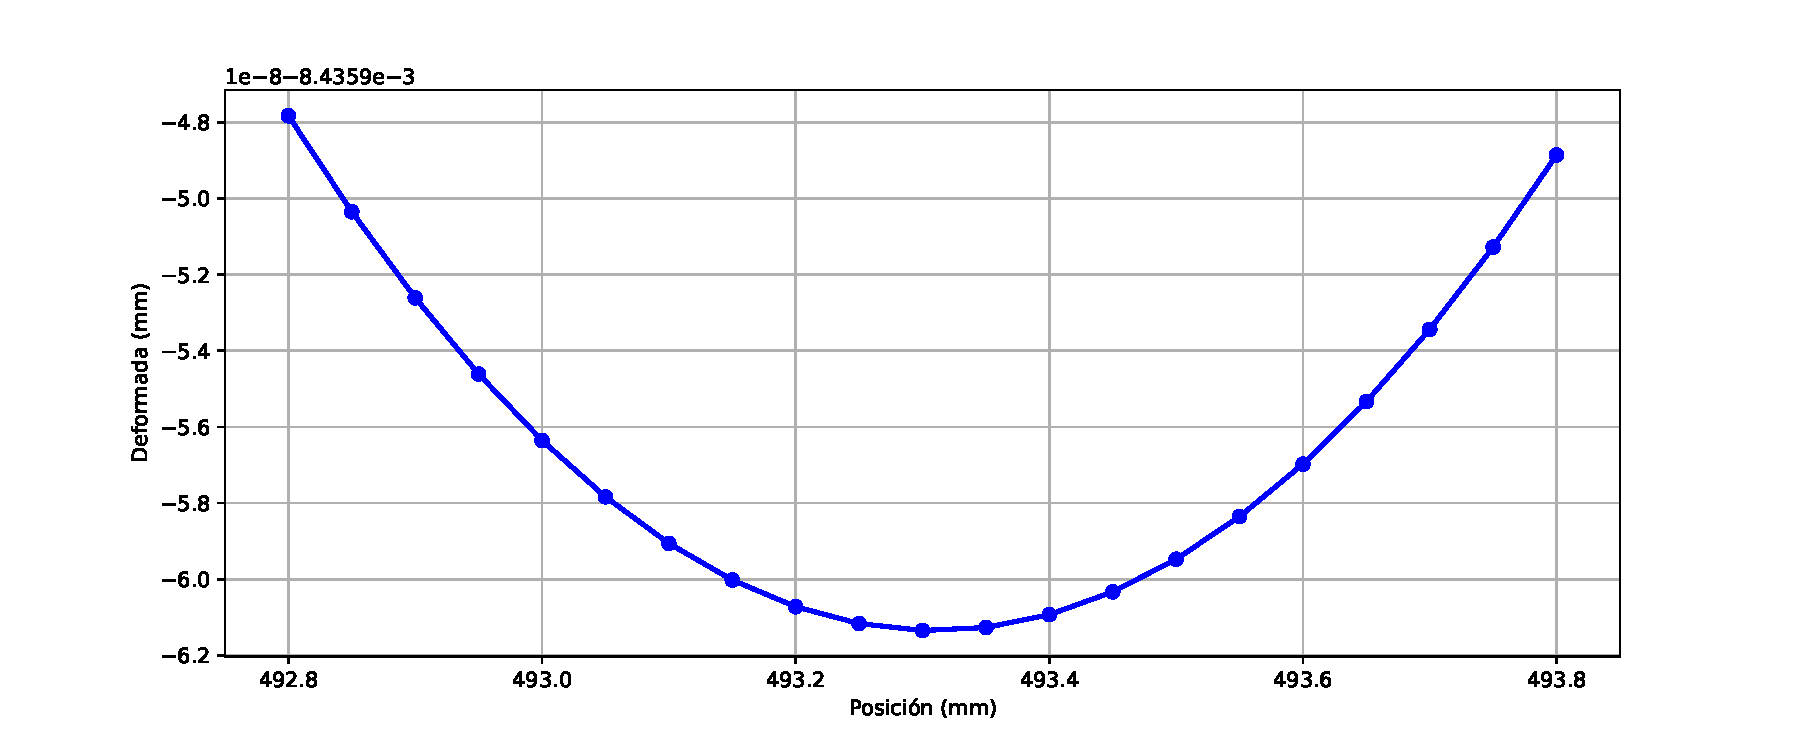
\includegraphics[scale=0.7]{refinament1.pdf}
    \caption{Refinamiento del mallado entre 490 y 500 mm}
\end{figure}
La flecha máxima está alrededor de 493.3 y tiene un valor de 0.0084359 mm, similar al resultado obtenido de forma analítica.
\subsection*{Análisis por diferencias finitas}
La viga también puede realizarse al seguir un procedimiento similar a como se hizo para el curso MC325, donde se puede usar el método de diferencias finitas para obtener una solución aproximada de la ecuación diferencial de la deformada. 
\begin{figure}[H]
    \centering
    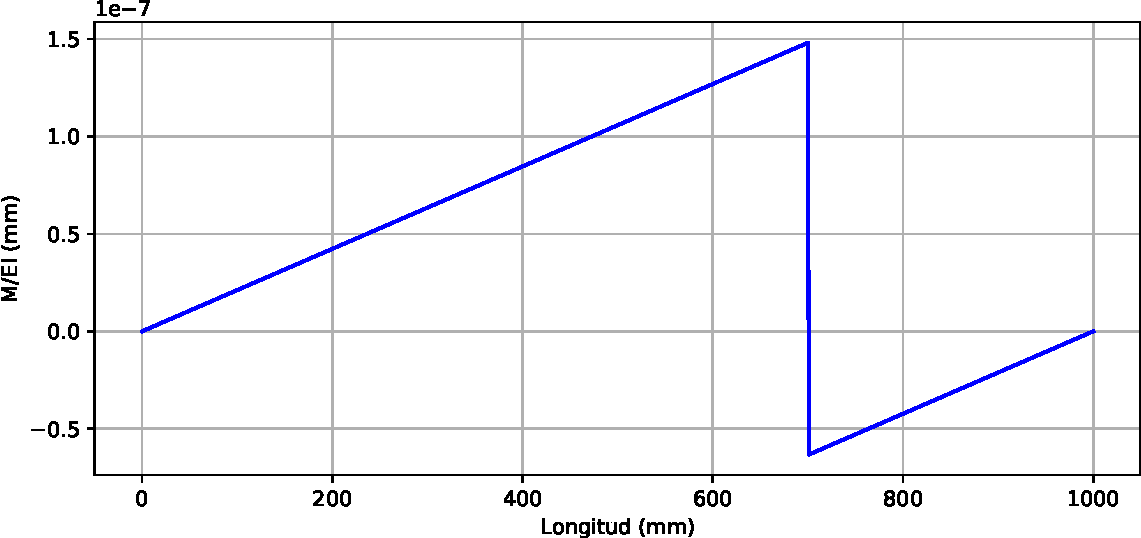
\includegraphics[scale=0.8]{mei.pdf}
    \caption{M/EI}
\end{figure}
\begin{figure}[H]
    \centering
    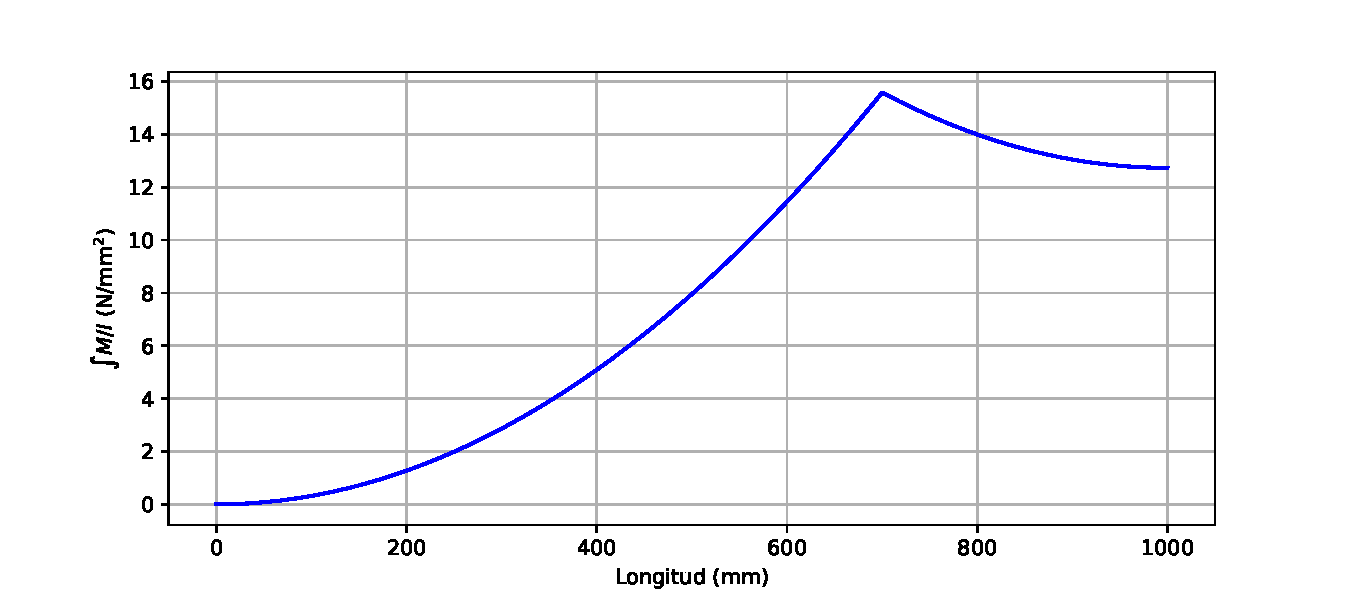
\includegraphics[scale=0.8]{mi.pdf}
    \caption{$\int M/I$}
\end{figure}
\begin{figure}[H]
    \centering
    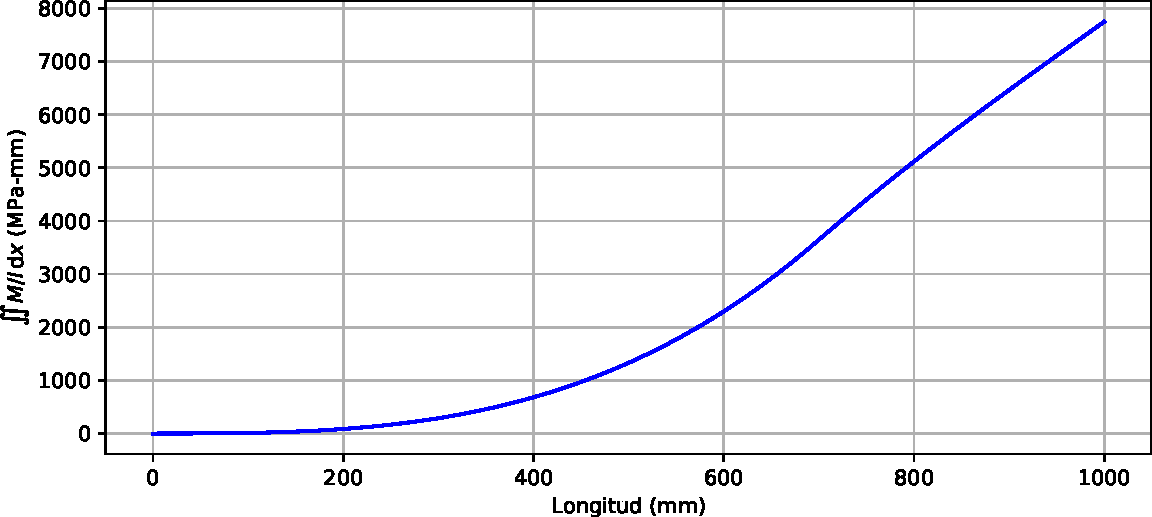
\includegraphics[scale=0.8]{mii.pdf}
    \caption{$\iint M/I$}
\end{figure}
Dado que la integral $\iint M/I$ contiene constantes, es necesario hallarlas y añadirlas a la gráfica final para obtener la deformada:
\begin{figure}[H]
    \centering
    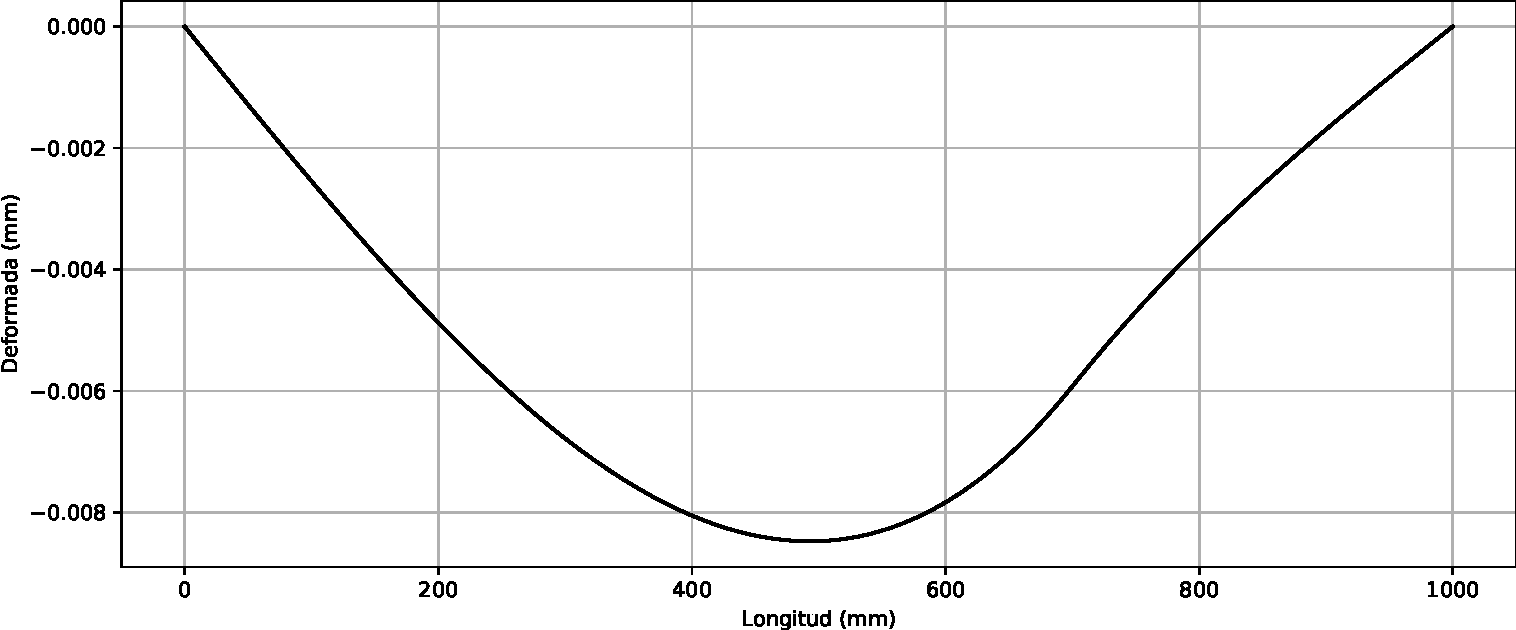
\includegraphics[scale=0.66]{deformada1000.pdf}
    \caption{Deformada obtenida por diferencias finitas}
\end{figure}
\subsection*{Comparación entre diferencias finitas y elementos finitos}
El método de diferencias finitas es la implementación de un clásico algoritmo DP, en el que se reutiliza estados anteriores para formar nuevos y así completar la solución completa. En este caso el algoritmo utiliza el estado anterior para así reconstruir la solución; es decir, es el método de Euler para la solución de una ecuación diferencial. Este método tiene una complejidad de tiempo $O(n)$ y la memoria puede optimizarse a $O(1)$, pero su convergencia a la solución es $O(n)$. Existen métodos más eficientes que utilizan aproximaciones más exactas para obtener una convergencia de $O(n^{2})$. Mientras que el método de elementos finitos aproxima la región obteniendo una convergencia igual al grado de la solución analítica, es decir $O(n^{3}/6)$ pero con un uso de memoria $O(n^{2})$ y un tiempo de ejecución de $O(n^{3})$, con las optimizaciones que se realizan en el código fue posible reducir el tiempo de ejecución a $O(n^{2}\log(n))$. Existen optimizaciones más poderosas para elementos finitos que reducen el uso de memoria excesivo usando una estructura de datos que elimina regiones de la matriz que son iguales a 0, de esa forma es posible usar más elementos y segmentar la solución.
\begin{figure}[H]
    \centering
    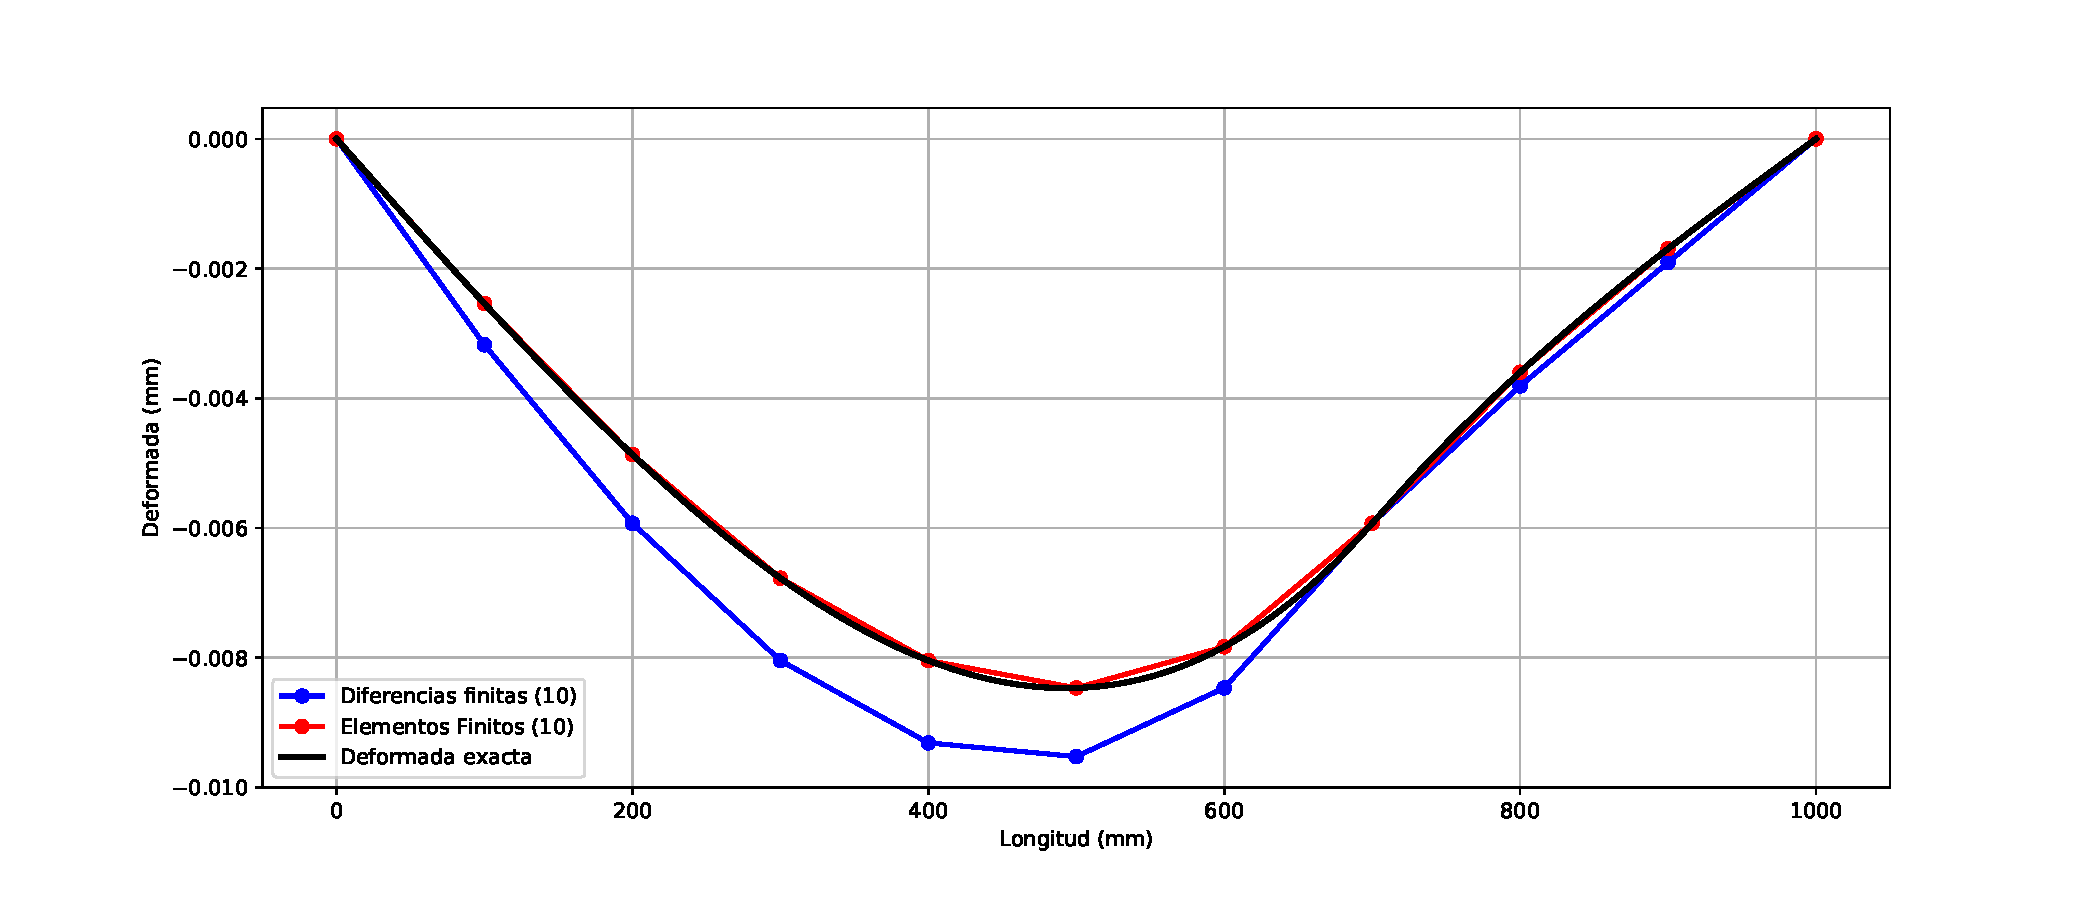
\includegraphics[scale=0.6]{comparision.pdf}
    \caption{Comparación entre el método de diferencias finitas y elementos finitos}
\end{figure}
Como tal, el método de elementos finitos presenta un mejor desarrollo para resolver problemas donde la convergencia obtenida puede ser muy alta, como es el caso de la viga. Esto puede observarse en la siguiente gráfica:

El método de elementos finitos con solo 10 elementos está más cerca a la deformada que el método de diferencias finitas con la misma cantidad; se observa que para obtener una convergencia similar sería necesario usar alrededor de 1000 elementos en diferencias finitas, haciendo que el método de elementos finitos sea mucho más eficiente.

\begin{table}[H]
    \centering
    \tcbox[left=0mm,right=0mm,top=0mm,bottom=0mm,boxsep=0mm,toptitle=0.8mm,bottomtitle=0.8mm,title=Elementos finitos y Diferencias finitas]{
    \renewcommand{\arraystretch}{1.2}%
    \begin{tabular}{c||c|c}
        \textbf{Características} & \textbf{Diferencias finitas} & \textbf{Elementos finitos}\\
        \hline
        \textbf{Tiempo de ejecución} & $O(n)$ & $O(n^{2}\log(n))$ \\
        \hline
        \textbf{Uso de memoria} & $O(1)$ & $O(n^{2})$ \\
        \hline
        \textbf{Convergencia} & $O(n)$ & $O(n^{3})$
    \end{tabular}}
    \caption{Comparación entre Elementos finitos y Diferencias finitas}
\end{table}
Además, existen métodos numéricos que pueden obtener una convergencia similar a elementos finitos con un tiempo de ejecución similar, dichos métodos son llamados multilinear-step y son usados como una generalización al método de Euler. 
\begin{thebibliography}{9}
\bibitem{d1} Optimized methods in FEM:\\
https://www.sciencedirect.com/topics/engineering/gauss-seidel-method
\bibitem{d3}
Sparse Matrix:\\
https://en.wikipedia.org/wiki/Sparse$\_$matrix
\bibitem{d4}
Sparse Matrix Library:\\
https://github.com/uestla/Sparse-Matrix
\bibitem{d5}
Mailman algorithm:\\
http://www.cs.yale.edu/homes/el327/papers/matrixVectorApp.pdf
\bibitem{d6}
Fast Algorithms with Preprocessing for Matrix-Vector Multiplication Problems:\\
https://www.sciencedirect.com/science/article/pii/S0885064X84710211
\end{thebibliography}
\end{document}
